% Section 2: model. Numbers: generated/numbers.tex; tables: ../results/tables/*.tex.
\section{Vehicle--track model}\label{sec:model}

\subsection{Wheelset and the effective support stiffness}\label{sec:wheelset}
The wheelset is a stepped Timoshenko beam (axle body, wheel seats, dust-guard collars and journals)
discretised with \NElements{} two-node elements with interdependent interpolation, which are free of
shear locking~\citep{friedman1993}. The shear coefficient is Cowper's value for a solid circular
section~\citep{cowper1966}. Each wheel is a rigid disc with mass and diametral inertia at its seat.
Each axlebox is a rigid mass on its journal, tied to a bogie frame that is held fixed by a linear
primary spring--damper pair. Axle damping is stiffness proportional. The model is linear and
vertical-plane. Gyroscopic and rotating-damping terms are omitted: the rotation rate is
\GyroRatio{} of the first constrained bending frequency at the reference speed (Table~\ref{tab:table2_verification}).

Between each journal and its axlebox the model has one spring--damper pair, $k_B$ and $c_B$. We call
$k_B$ the \emph{effective support stiffness}: the stiffness of the load path from journal to axlebox,
that is, the roller contacts of the bearing in series with the bearing housing, the adapter and any
pad,
\begin{equation}
  k_B(W, c) = \left[\frac{1}{k_\mathrm{contact}(W, c)} + \frac{1}{k_\mathrm{housing}}\right]^{-1},
  \label{eq:series}
\end{equation}
where $W$ is the axle load and $c$ the diametral clearance of the bearing. The quantity monitored in
this paper is a loss of $k_B$. It covers loosening of the bearing fits, degradation of the housing,
adapter or pad, and growth of the bearing clearance. It is not a model of rolling-contact fatigue
or spalling, which act at much higher frequencies through impacts.

\paragraph{Roller contacts.} For a double-row roller bearing under a static radial load, the
contact stiffness follows from the line-contact law of the wheelset model, $Q = K_n\,\delta^{10/9}$,
with the load shared over the rollers in the load zone (roller deflection
$\delta_j = \Delta\cos\theta_j\cos\alpha - c/2$, contact force summed over both rows; inner and
outer contacts in series; \citealp{harris2006}). For a generic freight unit
(placeholder geometry, \RollersPerRow{} rollers per row, initial clearance \ClearanceZero~\textmu m;
Table~\ref{tab:table1_parameters}) the cage-averaged contact stiffness is
\KcontactEmpty{} and \KcontactLoaded{}~GN/m per bearing at the empty and loaded axle loads.
These values are 6--8 times the nominal effective support stiffness of \kBnom~GN/m used throughout
(a placeholder), so in reading~\eqref{eq:series} the housing path carries most of the compliance.
A change of the contact stiffness then reaches $k_B$ diluted by the factor $k_B/k_\mathrm{contact}$,
\DilutionEmpty{} (empty) to \DilutionLoaded{} (loaded): a clearance growth of 10~\textmu m lowers the
contact stiffness by \ContactPctTenEmpty\% (empty) and \ContactPctTenLoaded\% (loaded), and $k_B$ by
\EffPctTenEmpty\% and \EffPctTenLoaded\%.

If instead $k_B$ were the contact stiffness alone, the axlebox-on-bearing resonance would sit near
\AxleboxModeContactHz~Hz (single-mass estimate with the \AxleboxMass~kg axlebox), where contact
filtering, the rail pinned--pinned mode and the flexible modes of the wheels, none of which the
model contains, dominate; that reading is outside the scope of this paper.

\paragraph{Load dependence.} The default stiffness law used for all results is the power law
\begin{equation}
  k_B(W) = k_{B0}\,(W/W_0)^{p},\qquad p = \LoadExp,
  \label{eq:powerlaw}
\end{equation}
the exponent of a line contact at zero clearance, with $W_0$ the loaded axle load and $k_{B0}$ the
health parameter. The series law~\eqref{eq:series}, with $k_\mathrm{housing}$ set so that
$k_B(W_0, c_0) = k_{B0}$, is implemented as an option; its effective exponent over the payload range
is \PeffSeries{}. The exponent is held fixed in the estimator; Section~\ref{sec:limitations}
discusses why it does not serve as a second, clearance-specific indicator.

\subsection{Rail, contact and multi-wheel coupling}\label{sec:rail}
The rail is an infinite Timoshenko beam on a continuous foundation of complex stiffness per unit
length $k_f(1+\mathrm{i}\eta_f)$. Its point and transfer receptances $R(x)$ follow in closed form by
partial fractions of the wavenumber-domain solution; the result equals Eq.~(11) of
Carrigan and Talbot~\citep{carrigan2023} and is checked against a numerical inverse transform. Rail
and foundation values are those of their Table~1 (BS113A rail, $k_f$ from their Sect.~5.1.1).
Each wheel meets the rail through a linearised Hertzian spring
$k_H = k_{H0}(W/W_0)^{1/3}$~\citep{carrigan2023}.

The instrumented wheelset runs with neighbouring wheels at positions $d_k$ along the same rail.
With $\mathbf{A}^w$ the wheel receptances, $\mathbf{A}^c = \mathrm{diag}(1/k_H)$ and
$A^r_{jk} = R(|d_j-d_k|)$, the contact forces under a roughness $z(x)$ are
\begin{equation}
  \mathbf{F} = (\mathbf{A}^c + \mathbf{A}^r + \mathbf{A}^w)^{-1}\mathbf{Z},\qquad
  Z_k = Z\,e^{\mathrm{i}\omega d_k/V},
  \label{eq:coupling}
\end{equation}
\citep[Eqs.~5 and 8]{carrigan2023}, and the axle-box acceleration per unit roughness at the
instrumented wheel is
\begin{equation}
  H(f;\bm\theta, W, V) = \sum_k G_k(f;\bm\theta, W)\,e^{\mathrm{i}2\pi f d_k/V}.
  \label{eq:H}
\end{equation}
Carrigan and Talbot drop the phase factors (their Eq.~6) because their spectra cannot resolve
them. We keep them: with records of \NumRevs{} wheel revolutions the frequency resolution resolves
the ripples of period $V/(d_k-d_j)$ (Fig.~\ref{fig:transfer}), and Section~\ref{sec:debias}
handles their effect on the likelihood. The default configuration has four wheels (the
instrumented bogie and the next), with the wheel layout of~\citep{carrigan2023} as a configuration
parameter.

\begin{figure}[tbp]\centering
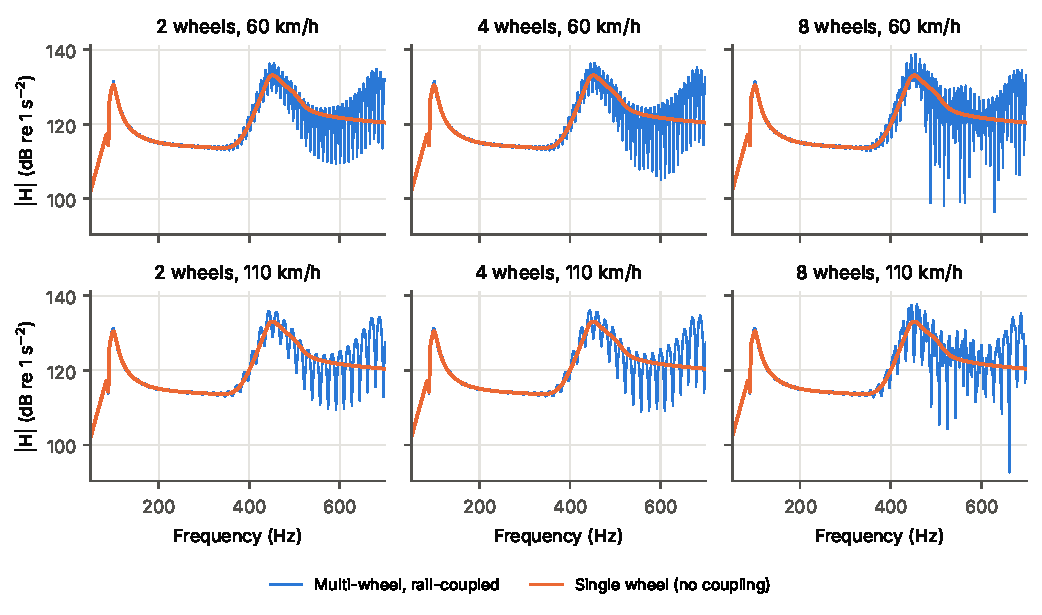
\includegraphics[width=\textwidth]{fig1_transfer_functions}
\caption{Axle-box acceleration per unit roughness, $|H|$, for 2, 4 and 8 rail-coupled wheels against
a single wheel without coupling, at 60 and 110~km/h. Data: \texttt{results/p2/fig1\_transfer.json}.}
\label{fig:transfer}
\end{figure}

\subsection{Verification}\label{sec:verification}
Table~\ref{tab:table2_verification} lists the checks of the reference model: free--free Timoshenko
frequencies against the closed form, the windowed energy balance of the steady-state solution,
frequency- against time-domain response, and mesh convergence. Unit tests cover the rail
receptance against Eq.~(11) of~\citep{carrigan2023} and the numerical inverse transform, and the
identity of the single-wheel coupled model with the rail-oscillator model.

% generated by experiments/make_tables.py from config/params.yaml, config/track.yaml; do not edit
\begin{table}[tbp]\centering\scriptsize
\caption{Model parameters and sources}\label{tab:table1_parameters}
\resizebox{\textwidth}{!}{\begin{minipage}{1.6\textwidth}\centering
\begin{tabular}{lllll}
\toprule
Group & Parameter & Value & Unit & Source \\ \midrule
Material & E & 2.10e11 & Pa & doc \S{}16 (standard steel) \\
Material & nu & 0.3 & - & doc \S{}16 \\
Material & rho & 7850 & kg/m\textasciicircum{}3 & doc \S{}16 \\
Axle & length & 2.18 & m & placeholder: typical standard-gauge freight axle \\
Axle & sections [outer $\xi$, d] & [[0.64,0.175],[0.86,0.2],[0.9,0.16],[1.09,0.13]] & m & placeholder: body / wheel seat / dust-guard collar / journal, typical EN 13103-type proportions \\
Axle & wheel\_xi & 0.75 & m & placeholder: contact plane \textasciitilde{} half of 1.5 m contact-point spacing \\
Axle & journal\_xi & 0.995 & m & placeholder: mid-journal bearing centre \\
Axle & n\_elements & 32 & - & brief: 20-40 elements; convergence checked at 20/30/40 \\
Axle & damping\_zeta & 0.01 & - & placeholder: 1\% stiffness-proportional at f\_ref \\
Axle & damping\_fref & 80 & Hz & placeholder: typical first wheelset bending frequency \\
Wheel & mass & 350 & kg & placeholder: 920 mm freight wheel \\
Wheel & diametral\_inertia & 20 & kg m\textasciicircum{}2 & placeholder: disc estimate m r\textasciicircum{}2/4 with rim correction \\
Wheel & r0 & 0.4575 & m & doc \S{}13 (new 915 mm wheel) \\
Bearing & kB0 & 1.0e9 & N/m & placeholder: tapered roller unit radial stiffness, order 1e8-1e9 \\
Bearing & cB & 5.0e3 & N s/m & placeholder: EHL/structural damping \\
Bearing & load\_exponent & 0.1 & - & doc Eq. (12): Q \textasciitilde{} delta\textasciicircum{}(10/9) gives k \textasciitilde{} Q\textasciicircum{}(1/10) \\
Axlebox & mass & 60 & kg & placeholder: housing + outer ring + adapter \\
Primary & kp & 1.0e6 & N/m & placeholder: freight primary vertical stiffness per axlebox \\
Primary & cp & 1.0e4 & N s/m & placeholder: equivalent linear damping per axlebox \\
Payload & W\_min & 5.5 & t & placeholder: empty freight wagon axle load \\
Payload & W\_max & 22.5 & t & placeholder: loaded (22.5 t axle load class) \\
Payload & W0 & 22.5 & t & reference load for kB0 (loaded) \\
Rail BS113A & A & 0.00717 & m\textasciicircum{}2 & CT23 Table 1 \\
Rail BS113A & rho & 7850 & kg/m\textasciicircum{}3 & CT23 Table 1 \\
Rail BS113A & E & 207.0e9 & Pa & CT23 Table 1 \\
Rail BS113A & I & 2.35e-05 & m\textasciicircum{}4 & CT23 Table 1 \\
Rail BS113A & G & 81.0e9 & Pa & CT23 Table 1 \\
Rail BS113A & kappa & 0.34 & - & CT23 Table 1 \\
Rail 60E1 & A & 0.00767 & m\textasciicircum{}2 & verify: EN 13674-1 60E1 section area 76.70 cm\textasciicircum{}2 (quoted from memory) \\
Rail 60E1 & I & 3.038e-05 & m\textasciicircum{}4 & verify: EN 13674-1 60E1 vertical-bending I\_x 3038.3 cm\textasciicircum{}4 (quoted from memory) \\
Foundation & standard\_kf\_lab & 154.0e6 & N/m\textasciicircum{}2 & CT23 Sec. 5.1.1: \textasciitilde{}100 MN/m per fastener (lab, Thompson et al.) at 0.65 m spacing \\
Foundation & resilient\_kf & 7.7e6 & N/m\textasciicircum{}2 & CT23 Sec. 5.1.1 (pass-by rail deflection, Cox \& Wang) \\
Foundation & eta\_f & 0.2 & - & CT23 Table 1 / Sec. 5.1.1 (literature range 0.2-0.3) \\
Contact & C\_H & 89.0e9 & N/m\textasciicircum{}1.5 & CT23 Sec. 5.1.2 citing Sanchis et al. (metro wheel/rail radii; freight wheel and 60E1 head radii differ: verify) \\
Layout & positions & [0.0,2.05,6.52,8.57,16.62,18.67,23.14,25.19,33.24,35.29,39.76,41.81] & m & CT23 Sec. 5.1.3 / Fig. 5: axle spacing 2.05, bogie centres 10.10 within a car, 6.52 across a coupling (positions derived from these) \\
\bottomrule
\end{tabular}

\par\smallskip{\footnotesize 15 of 35 entries are placeholders. Vehicle masses (wheel, axlebox, unsprung) stay placeholders until the target vehicle is confirmed; values marked 'verify' are to be checked against the cited standard.}
\end{minipage}}
\end{table}

% generated by experiments/make_tables.py from results/p1/verification.json, results/gates/G1.json; do not edit
\begin{table}[tbp]\centering\scriptsize
\caption{Verification of the reference model}\label{tab:table2_verification}
\resizebox{\textwidth}{!}{\begin{minipage}{1.6\textwidth}\centering
\begin{tabular}{llll}
\toprule
Check & Measured & Threshold & Gate \\ \midrule
Free--free Timoshenko frequencies vs closed form (max rel. error, 4 modes) & 3.62e-03 & 5e-03 & PASS \\
Energy balance, windowed integral (max rel. residual, 3 cases) & 1.3e-11 & 1e-06 & PASS \\
Frequency vs time domain, axlebox accel. (max rel. L2, 3 cases) & 1.8e-06 & 1e-03 & PASS \\
Mesh 20 vs 40 elements, modes (max rel. diff.) & 2.0e-03 & -- & -- \\
Gyroscopic neglect, $\Omega$/$\omega$$_1$ & 0.106 & -- & -- \\
\bottomrule
\end{tabular}

\par\smallskip{\footnotesize Rail receptance vs CT23 Eq. 11 and the numerical inverse transform, and the single-wheel coupling identity (1e-9), are unit tests in tests/test\_track.py (all pass).}
\end{minipage}}
\end{table}

